\documentclass{beamer}
\usetheme[compress]{Berlin}
\usecolortheme{dolphin}
\usepackage{lmodern}
\usepackage{amsmath}
\usepackage{amsthm}
\usepackage{amssymb}
\usepackage{enumerate}
\usepackage{mathtools}
\usepackage{mathrsfs}
\usepackage{tikz}

\title{Generalising induction, and coinduction}
\author{Bhavik Mehta}
\institute{Part III Seminar}
\date{Friday 30 November}

\DeclareMathOperator{\ob}{ob}
\DeclareMathOperator{\mor}{mor}
\newcommand{\cc}{\mathscr{C}}

\usetikzlibrary{cd, decorations.text}
\tikzset{
    dot/.style={fill=black, circle, inner sep=1pt},
    invisible/.style={opacity=0},
    visible on/.style={alt={#1{}{invisible}}},
    alt/.code args={<#1>#2#3}{%
      \alt<#1>{\pgfkeysalso{#2}}{\pgfkeysalso{#3}}%
  }
}

\begin{document}
% automata as coalgebra
% naturals as algebra/ conaturals as coalgebra
% [0,1] as terminal coalgebra (julia set?)
% trees as coalgebra
% list as algebra
% polynomial functors giving languages
\begin{frame}
  \titlepage
\end{frame}
\begin{frame}
  \frametitle{Generalising induction, and coinduction}
  \begin{itemize}
    \item<2-> Recursive definitions and principle of induction away from $\mathbb{N}$
    \item<3-> Dualise: what is corecursive data?
      \vspace{\baselineskip}
    \item<4-> Universal algebra, model theory, automata, real analysis, theoretical computer science
  \end{itemize}
\end{frame}
\section{Algebras and coalgebras}
\subsection{Definitions}
\begin{frame}[fragile]
  \frametitle{Algebras of an endofunctor}
  Take an endofunctor $F :\mathscr{C} \to \mathscr{C}$
  \begin{definition}[$F$-algebra]
    An $F$-algebra is a pair $(A,\,\alpha: FA \to A)$ with $A \in \ob \mathscr{C}$
  \end{definition}
  \pause
  \begin{definition}[Algebra homomorphism]
    A homomorphism of $F$-algebras $(A,\alpha) \to (B,\beta)$ is a morphism $f: A \to B$ with
    \begin{equation*}
      \begin{tikzcd}[cramped]
        FA \rar{Ff} \dar{\alpha} & FB \dar{\beta} \\
        A \rar{f} & B
      \end{tikzcd}
    \end{equation*}
  \end{definition}
  $\mathbf{Alg} F$ is the category of $F$-algebras
\end{frame}
\begin{frame}[fragile]
  \frametitle{\alert{Co}algebras of an endofunctor}
  Take an endofunctor $F :\mathscr{C} \to \mathscr{C}$
  \begin{definition}[$F$-\alert{co}algebra]
    An $F$-\alert{co}algebra is a pair $(A,\,\alpha: A \to FA)$ with $A \in \ob \mathscr{C}$
  \end{definition}
  \begin{definition}[\alert{Co}algebra homomorphism]
    A homomorphism of $F$-coalgebras $(A,\alpha) \to (B,\beta)$ is a morphism $f: A \to B$ with
    \begin{equation*}
      \begin{tikzcd}[cramped]
        A \rar{f}\dar{\alpha}  & B \dar{\beta} \\
        FA \rar{Ff} & FB
      \end{tikzcd}
    \end{equation*}
  \end{definition}
  $\mathbf{Coalg} F$ is the category of $F$-coalgebras
\end{frame}
\subsection{Examples}
\begin{frame}
  \frametitle{``Monoids''}
  \onslide<1->{
    \begin{center}
      $FX \coloneqq 1 + X \times X$
  \end{center}}
  \begin{columns}
    \begin{column}{0.4\textwidth}
      \begin{gather*}
        \onslide<1->{
          \begin{tikzcd}[ampersand replacement=\&, column sep=small]
            1 \rar \arrow[dr,"e"'] \& {\scriptstyle 1 + A \times A} \dar[dashed,pos=0.4]{\scriptscriptstyle e+m} \& A \times A \lar \arrow[ld,"m"] \\
            \& A
          \end{tikzcd}
        }
        \\\\
        \onslide<3->{
          \begin{tikzcd}[ampersand replacement=\&, column sep=small]
            \scriptstyle{1 + A \times A} \rar \dar[']{\scriptscriptstyle e_A + m_A} \& \scriptstyle{1 + B \times B} \dar{\scriptscriptstyle e_B + m_B} \\
            A \rar[']{f} \& B
          \end{tikzcd}
        }
      \end{gather*}
    \end{column}
    \begin{column}{0.6\textwidth}
      \begin{itemize}
        \item \onslide<2->{An $F$-algebra gives an \emph{interpretation}, not necessarily a model}
          \begin{align*}\onslide<3->{
              f(e_A) &= e_B \\
              f(m_A(x,y)) &= m_B(f(x),f(y))}
          \end{align*}
        \item \onslide<4->{$\mathbf{Alg}F$ has a full subcategory isomorphic to $\mathbf{Mon}$}
      \end{itemize}
    \end{column}
  \end{columns}
\end{frame}
\begin{frame}[fragile]
  \frametitle{Trees}
  \begin{itemize}[<+->]
    \item
      The set $T$ of finite binary trees gives an $F$-algebra
      \begin{equation*}
        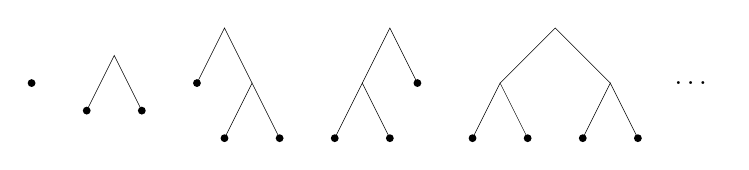
\begin{tikzpicture}[scale=0.7]
          \begin{scope}
            \node [dot] at (0,0.5) {};
          \end{scope}
          \begin{scope}[xshift=1cm]
            \node [dot] at (0,0) {};
            \node [dot] at (1,0) {};
            \draw [very thin] (0,0) -- (0.5,1) -- (1,0);
          \end{scope}
          \begin{scope}[xshift=3.5cm, yshift=-0.5cm]
            \node [dot] at (-0.5,1) {};
            \node [dot] at (0,0) {};
            \node [dot] at (1,0) {};
            \draw [very thin] (0,0) -- (0.5,1) -- (1,0);
            \draw [very thin] (-0.5,1) -- (0,2) -- (0.5,1);
        \end{scope}
        \begin{scope}[xshift=5.5cm, yshift=-0.5cm]
          \node [dot] at (1.5,1) {};
          \node [dot] at (0,0) {};
          \node [dot] at (1,0) {};
          \draw [very thin] (0,0) -- (0.5,1) -- (1,0);
          \draw [very thin] (1.5,1) -- (1,2) -- (0.5,1);
        \end{scope}
        \begin{scope}[xshift=8cm, yshift=-0.5cm]
          \node [dot] at (0,0) {};
          \node [dot] at (1,0) {};
          \node [dot] at (2,0) {};
          \node [dot] at (3,0) {};
          \draw [very thin] (0,0) -- (0.5,1) -- (1,0);
          \draw [very thin] (0.5,1) -- (1.5,2) -- (2.5,1);
          \draw [very thin] (2,0) -- (2.5,1) -- (3,0);
        \end{scope}
        \node at (12,0.5) {$\dotsc$};
      \end{tikzpicture}
    \end{equation*}
    $1 \to T$ gives empty tree, $T \times T \to T$ combines trees
    \item All binary trees also works
  \end{itemize}
\end{frame}
\begin{frame}
  \frametitle{More algebra examples}
  \begin{itemize}[<+->]
    \item $FX \coloneqq 1 + X + X \times X$

      $FA \to A$ decomposes into $1 \to A$, $A \to A$, $A \times A \to A$
    \item $FX \coloneqq X \times X$ has semigroups, $FX \coloneqq 2 + X + 2 \times X \times X$ has rings
    \item $FX \coloneqq \mathcal{P}X$, then $\mathcal{P}A \to A$ could be a point in $A$, or $\mathcal{P}\mathcal{P}B \to \mathcal{P}B$, or many things...
    \item If $F 0 = 0$ then $0$ has an $F$-algebra structure
  \end{itemize}
\end{frame}
\begin{frame}
  \frametitle{Coalgebra examples}
  \begin{itemize}
    \item<1-> $FX = 1 + X$, then $f: A \to 1 + A$
      \begin{center}
        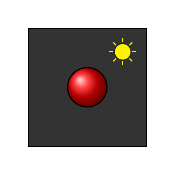
\begin{tikzpicture}
          \draw [fill=black!80!white] (0,0) rectangle (1.5,1.5);
          \draw [shade, shading=ball, ball color=red] (0.75,0.75) circle (0.25cm);
          \draw [fill=white!80!yellow] (1.2,1.2) circle (0.1cm);
          \only<2->{
            \fill [yellow] (1.2,1.2) circle (0.1cm);
            \foreach \x in {0,45,...,315} {
              \draw [yellow] (1.2,1.2) ++(\x:0.12) -- ++(\x:0.05);
            }
          }
        \end{tikzpicture}
      \end{center}
    \item<3-> $FX \coloneqq B \times X$, then $A \to B \times A$ is a deterministic automaton with output in $B$ (but no fixed input state)
    \item<4-> $FX \coloneqq \mathcal{P}X$ models non-deterministic automata
    \item <5-> $FX \coloneqq 1 + X \times X$
      \begin{center}
        
\begin{tikzpicture}
          \draw [fill=black!80!white] (0,0) rectangle (1.5,1.5);
          \draw [fill=red!80!white] (0.6,0.5) -- (0.6,1) -- (0.3,0.75) -- cycle;
          \draw [fill=red!80!white] (0.9,0.5) -- (0.9,1) -- (1.2,0.75) -- cycle;
          \draw [fill=white!80!yellow] (1.2,1.2) circle (0.1cm);
        \end{tikzpicture}
      \end{center}
      and trees
  \end{itemize}
\end{frame}

\section{Initiality}
\subsection{Initial algebras}
\begin{frame}[fragile]
  \frametitle{Initial algebras}
  \begin{definition}
    An initial $F$-algebra is an initial object in the category of $F$-algebras
  \end{definition}
  For any $FA \to A$, there is a unique morphism $i: I \to A$, with
  \begin{equation*}
  \begin{tikzcd}
    FI \rar{Fi} \dar & FA \dar \\
    I \rar{i} & A
  \end{tikzcd}
  \end{equation*}
  \pause
  \begin{definition}
    A terminal (or final) $F$-coalgebra is a terminal object in the category of $F$-coalgebras
  \end{definition}
\end{frame}
\subsection{Examples}
\begin{frame}[fragile]
  \frametitle{Induction on $\mathbb{N}$}
  Take $FX = 1 + X$ on $\mathbf{Set}$, then $\mathbb{N}$ forms an $F$-algebra
  \begin{equation*}
    \begin{tikzcd}
      1 \rar \drar[']{0} & 1 + \mathbb{N} \dar[dashed]{0+s} & \lar \mathbb{N} \arrow[ld, "s"]\\
             & \mathbb{N}
    \end{tikzcd}
  \end{equation*}
  \pause
  \begin{equation*}
    \begin{tikzcd}
      1 + \mathbb{N} \rar{1 + \varphi} \dar{0 + s} & 1 + A \dar{x_0 + f}\\
      \mathbb{N} \rar{\varphi} & A
    \end{tikzcd}
    \qquad
    \begin{aligned}
      \varphi(0) &= x_0 \\
      \varphi(n+1) &= f(\varphi(n))
    \end{aligned}
  \end{equation*}
  Recall: Subobjects of an initial object are isomorphic to it
\end{frame}
\begin{frame}
  \frametitle{Streams}
  $FX = B \times X$, fixed set $B$; $B^\infty$ is infinite sequences (streams) of $B$;
  $B^\infty \to B \times B^\infty$ is head and tail, $(x_n)_{n=0}^\infty \mapsto \left( x_0, (x_n)_{n=1}^\infty\right)$
  \pause
  \begin{columns}
    \begin{column}{0.5\textwidth}
      \begin{equation*}
        \begin{tikzcd}[ampersand replacement=\&]
          A \rar{\varphi} \dar{f} \& B^\infty \dar \\
          B \times A \rar{1_B \times \varphi} \& B \times B^\infty
      \end{tikzcd}
    \end{equation*}
    \only<4->{Initial algebra is boring}
    \end{column}
    \begin{column}{0.5\textwidth}
      \begin{align*}
        a_0 &\mapsto (b_1, a_2) \\
        a_1 &\mapsto (b_3, a_0) \\
        a_2 &\mapsto (b_4, a_1)
      \end{align*}
      \vspace{-2em}
      \uncover<3->{
        \begin{align*}
          \varphi(a_0) &= \langle b_1 , \varphi(a_2) \rangle \\
                       &= \langle b_1, \langle b_4 , \varphi(a_1) \rangle \rangle \\
                       &= \langle b_1, \langle b_4, \langle b_3, \varphi(a_0) \rangle \rangle \rangle \\
                       &= (b_1, b_4, b_3, b_1, b_4, \dotsc)
        \end{align*}
      }
    \end{column}
  \end{columns}

\end{frame}
\begin{frame}[fragile]
  \frametitle{Powerset functors}
  $\mathcal{P}_\text{fin}$ on $\mathbf{Set}$ has an initial algebra $(V_\omega, \text{id})$, \alert{hereditarily finite sets}
  \begin{equation*}
    \begin{tikzcd}
      \mathcal{P}_{\text{fin}} V_\omega \dar{\text{id}} \rar{\mathcal{P}_{\text{fin}} \varphi} & \mathcal{P}_{\text{fin}} A \dar{f} \\
      V_\omega \rar{\varphi} & A
    \end{tikzcd}
  \end{equation*}
  \pause
  \begin{equation*}
    \varphi(x) = f(\{\varphi(s) : s \in x\})
  \end{equation*}
  \pause
  $\mathcal{P}_\kappa =$ subsets of cardinality $<\kappa$ has $V_\kappa$.
  What about $\mathcal{P}$ itself?
\end{frame}
\section{Fixed points}
\subsection{Lambek's Lemma}
\begin{frame}
  \frametitle{A necessary condition}
  \begin{lemma}[Lambek]
    If $(A, \alpha)$ is an initial $F$-algebra, then $\alpha$ is an isomorphism
  \end{lemma}
  \onslide<2->{
  \begin{proof}
    \begin{equation*}
      \begin{tikzcd}[ampersand replacement=\&,sep=large]
        FA \dar{\alpha} \rar[visible on=<3->]{Fi} \arrow[rd, visible on=<6->, "F1_{A}"]\& {\visible<3->{FFA}} \rar[visible on=<4->]{F\alpha} \arrow[visible on=<3->, d, "F\alpha"] \& {\visible<4->{FA}} \dar[visible on=<4->]{\alpha} \\
        A \rar[visible on=<3->]{i} \arrow[rr, visible on=<5->, "1_A", bend right,'] \& FA \rar[visible on=<4->]{\alpha} \& {\visible<4->{A}}
    \end{tikzcd}
    \end{equation*}
  \end{proof}
  }
\end{frame}
\begin{frame}
  \frametitle{Fixed points of an endofunctor}
  \begin{itemize}
    \item If $(A,\alpha)$ is initial, then $FA \cong A$
    \item Dually, if $(A, \alpha)$ is a terminal coalgebra, then $A \cong FA$.
  \end{itemize}
  \pause
  \begin{definition}[Fixed point]
    A fixed point of $F$ is an isomorphism $FA \to A$ (equivalently, $A \to FA$)
  \end{definition}
  \pause
  \begin{itemize}
    \item $\mathcal{P}$ has no fixed points, in particular no initial algebra (Cantor)
    \item If $0$ is a fixed point of $F$, it is an initial algebra
  \end{itemize}
\end{frame}
\begin{frame}
  \frametitle{Least, greatest fixed points}
  \begin{itemize}[<+->]
    \item $\operatorname{Fix}(F)$, a full subcategory of $\mathbf{Alg} F$ and of $\mathbf{Coalg} F$
    \item Initial algebra is initial in this subcategory
    \item Subobjects of an initial object are isomorphic to it
    \item So initial algebra is \emph{least} fixed point
    \item Dually, terminal coalgebra is greatest fixed point
  \end{itemize}
\end{frame}
\section{Recursion and induction}
\subsection{Trees}
\begin{frame}
  \frametitle{Trees}
      \begin{equation*}
        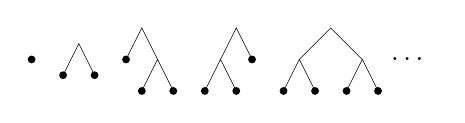
\begin{tikzpicture}[scale=0.4]
          \begin{scope}
            \node [dot] at (0,0.5) {};
          \end{scope}
          \begin{scope}[xshift=1cm]
            \node [dot] at (0,0) {};
            \node [dot] at (1,0) {};
            \draw [very thin] (0,0) -- (0.5,1) -- (1,0);
          \end{scope}
          \begin{scope}[xshift=3.5cm, yshift=-0.5cm]
            \node [dot] at (-0.5,1) {};
            \node [dot] at (0,0) {};
            \node [dot] at (1,0) {};
            \draw [very thin] (0,0) -- (0.5,1) -- (1,0);
            \draw [very thin] (-0.5,1) -- (0,2) -- (0.5,1);
          \end{scope}
          \begin{scope}[xshift=5.5cm, yshift=-0.5cm]
            \node [dot] at (1.5,1) {};
            \node [dot] at (0,0) {};
            \node [dot] at (1,0) {};
            \draw [very thin] (0,0) -- (0.5,1) -- (1,0);
            \draw [very thin] (1.5,1) -- (1,2) -- (0.5,1);
          \end{scope}
          \begin{scope}[xshift=8cm, yshift=-0.5cm]
            \node [dot] at (0,0) {};
            \node [dot] at (1,0) {};
            \node [dot] at (2,0) {};
            \node [dot] at (3,0) {};
            \draw [very thin] (0,0) -- (0.5,1) -- (1,0);
            \draw [very thin] (0.5,1) -- (1.5,2) -- (2.5,1);
            \draw [very thin] (2,0) -- (2.5,1) -- (3,0);
          \end{scope}
        \node at (12,0.5) {$\dotsc$};
      \end{tikzpicture}
    \end{equation*}

    \vspace{\baselineskip}
    $T$ is initial for $FX = 1 + X^2$
    \pause
    \begin{columns}
      \begin{column}{0.5\textwidth}
        \begin{equation*}
          \begin{tikzcd}[ampersand replacement=\&]
            1 + T^2 \rar \dar \& 1 + \mathbb{N}^2 \dar{1 + \textsf{add}} \\
            T \rar{\varphi} \uar[bend left, dashed] \& \mathbb{N}
          \end{tikzcd}
        \end{equation*}
      \end{column}
      \begin{column}{0.5\textwidth}
        \onslide<3->{
        \begin{align*}
          \varphi\left(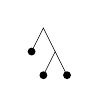
\begin{tikzpicture}[scale=0.3,baseline=5pt]
                \node [dot] at (-0.5,1) {};
                \node [dot] at (0,0) {};
                \node [dot] at (1,0) {};
                \draw [very thin] (0,0) -- (0.5,1) -- (1,0);
                \draw [very thin] (-0.5,1) -- (0,2) -- (0.5,1);
      \end{tikzpicture}\right) &= \varphi({\tikz[baseline=-2pt] \node[dot] at (0,0) {};})  + \varphi(
          
\begin{tikzpicture}[scale=0.3, baseline=1pt]
            \node [dot] at (0,0) {};
            \node [dot] at (1,0) {};
            \draw [very thin] (0,0) -- (0.5,1) -- (1,0);
          \end{tikzpicture}
      ) \\
                    &= 1 + (\varphi({\tikz[baseline=-2pt] \node[dot] at (0,0) {};})+\varphi({\tikz[baseline=-2pt] \node[dot] at (0,0) {};}))\\
                    &= 3.
        \end{align*}
      }
      \end{column}
    \end{columns}
\end{frame}
\begin{frame}
  \frametitle{Trees, continued}
    \begin{columns}
      \begin{column}{0.4\textwidth}
        \begin{gather*}
          \begin{tikzcd}[ampersand replacement=\&]
            1 + T^2 \rar \dar \& 1 + \mathbb{N}^2 \dar{0 + f} \\
            T \rar{\varphi} \uar[bend left, dashed] \& \mathbb{N}
          \end{tikzcd} \\
          f(m,n) = 1 + \max\{m,n\}
        \end{gather*}
      \end{column}
      \begin{column}{0.6\textwidth}
        \onslide<2->{
          \begin{align*}
            \varphi\left(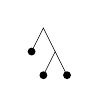
\begin{tikzpicture}[scale=0.3,baseline=5pt]
                \node [dot] at (-0.5,1) {};
                \node [dot] at (0,0) {};
                \node [dot] at (1,0) {};
                \draw [very thin] (0,0) -- (0.5,1) -- (1,0);
                \draw [very thin] (-0.5,1) -- (0,2) -- (0.5,1);
              \end{tikzpicture}\right) &= 1 + \max\{\varphi({\tikz[baseline=-2pt] \node[dot] at (0,0) {};}), \varphi(
              
\begin{tikzpicture}[scale=0.3, baseline=1pt]
                \node [dot] at (0,0) {};
                \node [dot] at (1,0) {};
                \draw [very thin] (0,0) -- (0.5,1) -- (1,0);
          \end{tikzpicture}
        )\} \\
                    &= 1 + (1 + \max \{\varphi({\tikz[baseline=-2pt] \node[dot] at (0,0) {};}),\varphi({\tikz[baseline=-2pt] \node[dot] at (0,0) {};})\})\\
                    &= 2.
          \end{align*}}
        \end{column}
    \end{columns}
\end{frame}
\subsection{}
\begin{frame}
  \frametitle{Conaturals?}
  $FX = 1 + X$. Take $\overline{\mathbb{N}} = \mathbb{N} \cup \{\infty\}$, and
  \begin{align*}
    \alpha: \overline{\mathbb{N}} &\longrightarrow 1 + \overline{\mathbb{N}}\\
    0 &\longmapsto * \\
    n &\longmapsto n-1 \\
    \infty &\longmapsto \infty
  \end{align*}
      \begin{columns}
        \begin{column}{0.5\textwidth}
          \begin{equation*}
            \begin{tikzcd}[ampersand replacement=\&]
              A \rar \dar \& \overline{\mathbb{N}} \dar \\
              1 + A \rar \& 1 + \overline{\mathbb{N}}
            \end{tikzcd}
          \end{equation*}
        \end{column}
        \begin{column}{0.5\textwidth}
          \begin{center}
            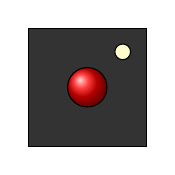
\begin{tikzpicture}
              \draw [fill=black!80!white] (0,0) rectangle (1.5,1.5);
              \draw [shade, shading=ball, ball color=red] (0.75,0.75) circle (0.25cm);
              \draw [fill=white!80!yellow] (1.2,1.2) circle (0.1cm);
            \end{tikzpicture}
          \end{center}
        \end{column}
      \end{columns}
\end{frame}
\begin{frame}
  \frametitle{Finite lists}
  $FX = 1 + B \times X$, $B^*$ are the finite sequences of $B$ (finite lists)
  \begin{columns}
    \begin{column}{0.45\textwidth}
  \begin{gather*}
    \onslide<2->{
    \begin{tikzcd}[ampersand replacement=\&]
      {\scriptstyle 1 + \mathbb{Z} \times \mathbb{Z}^*} \rar \dar[']{\varepsilon + \langle \cdot , \cdot \rangle } \& {\scriptstyle 1 + \mathbb{Z} \times \mathbb{Q}} \dar{f} \\
      \mathbb{Z}^* \rar{\varphi} \& \mathbb{Q}
    \end{tikzcd}
    \\
    \begin{aligned}
      f(*) &= 1 \\
      f(n, q) &= n \times q
    \end{aligned}}
  \end{gather*}
    \end{column}
    \begin{column}{0.55\textwidth}
      \begin{align*}
        \onslide<3->{
        \varphi([3,-4,2]) &= f(3, \varphi([-4,2])) \\
        \varphi([-4,2]) &= f(-4, \varphi([2])) \\
        \varphi([2]) &= f(2, \varphi([])) \\
        \varphi([]) &= f(*) = 1 \\
      }
        \onslide<4->{
        \varphi([3,-4,2]) &= 3 \times (-4 \times (2 \times 1)) \\
                          &= -24}
      \end{align*}
    \end{column}
  \end{columns}
\end{frame}
\begin{frame}
  \frametitle{More coalgebras}
  Terminal coalgebra of $FX = 1 + B \times X$ is (potentially infinite) lists, $B^{\omega}$
  \begin{columns}
    \begin{column}{0.45\textwidth}
      \begin{align*}
        \beta: B^\omega &\to 1 + B \times B^\omega \\
        \varepsilon &\mapsto * \\
        \langle b_0, \mathbf{b} \rangle &\mapsto (b_0, \mathbf{b})
      \end{align*}
      \onslide<2->{
      \begin{equation*}
        \begin{tikzcd}[ampersand replacement=\&, column sep=small]
          \mathbb{Z} \rar{\varphi} \dar{f} \& \mathbb{Z}^\omega \dar{\beta} \\
          1 + \mathbb{Z} \times \mathbb{Z} \rar \& 1 + \mathbb{Z} \times \mathbb{Z}^\omega\uar[dashed, bend left]
        \end{tikzcd}
      \end{equation*}
      }
    \end{column}
    \begin{column}{0.55\textwidth}
      \onslide<2->{
      \begin{align*}
        f(0) &= * \\
        f(n) &= (n, n-1)
      \end{align*} }%
      \onslide<3->{\vspace{-1.5em}%
      \begin{align*}
        \varphi(2) &= \langle 2, \varphi(1) \rangle \\
        &= \langle 2, \langle 1, \varphi(0) \rangle \rangle \\
        &= \langle 2, \langle 1, \varepsilon \rangle \rangle \\
        &= [2,1]
      \end{align*}
    $\varphi(-5)$ is infinite: $[-5, -6, -7, \dotsc]$}
    \end{column}
  \end{columns}
\end{frame}
\section{Summary}
\subsection{}
\begin{frame}
  \frametitle{Our examples}
  \begin{table}
    \begin{tabular}{c | c | c}
    Functor & Initial algebra & Terminal coalgebra \\
    \hline \hline
    $1 + X$ & naturals & conaturals \\
    $1 + X^2$ & finite binary trees & binary trees \\
    $1 + B \times X$ & finite lists & lists \\
    $B \times X$ & empty & streams \\
    $\mathcal{P}_{\text{fin}}$ & $V_\omega$ & finitely branching trees
    \end{tabular}
  \end{table}
  \pause
  \begin{itemize}[<+->]
    \item Dyadic rationals in $[0,1]$ as an initial algebra
    \item (Freyd) $[0,1]$ itself as a terminal coalgebra (as a set, poset, totally ordered set or topologically)
    \item (Leinster) $L^1[0,1]$ (with Lebesgue measure) as a terminal coalgebra, and Julia sets
  \end{itemize}
\end{frame}
\begin{frame}
  \frametitle{Sufficient conditions?}
  \begin{itemize}[<+->]
    \item Can have a least fixed point and no initial algebra
    \item But with some conditions on $\cc$ and $F$, $F$ has a fixed point iff an initial $F$-algebra exists
      \begin{itemize}
        \item for example, if $F$ preserves monomorphisms in $\mathbf{Set}, \mathbf{Top}$
      \end{itemize}
    \item But $F$ can preserve monomorphisms and have a fixed point, but no terminal coalgebra
      \begin{theorem}[Ad\'amek]
        Let $0$ be initial in $\cc$, and suppose
        \begin{equation*}
          \begin{tikzcd}[ampersand replacement=\&]
            0 \rar{!} \& F0 \rar{F!} \& F^2 0 \rar{F^2 !} \& \dots
          \end{tikzcd}
        \end{equation*}
        has a colimit, which is preserved by $F$. Then the colimit carries an initial algebra.
      \end{theorem}
  \end{itemize}
\end{frame}
\begin{frame}
  \frametitle{Recursion vs corecursion}
  \begin{itemize}
    \item Recursion allows defining a map out of a structure by reducing to easier cases
    \item Induction defines what to do on constructors
    \item Corecursion allows defining a map to a complex structure by building up from a seed
    \item Coinduction defines what destructors do
  \end{itemize}
\end{frame}
\begin{frame}
  \frametitle{Further reading}
  \begin{itemize}
    \item Initial algebras and terminal coalgebras: a survey (Ad\'amek, Milius, Moss)
    \item A study of categories of algebras and coalgebras (Hughes)
    \item A general theory of self-similarity (Leinster)
  \end{itemize}
\end{frame}
\appendix
\section{Appendix}
\subsection{}
\begin{frame}
  \frametitle{Sketch proof of Ad\'amek's Theorem}
        \begin{equation*}
          \begin{tikzcd}[ampersand replacement=\&, sep=large]
            0 \rar{!} \arrow[rd] \& F0 \rar{F!} \arrow[d] \& F^2 0 \rar{F^2 !} \arrow[ld] \& \dots \arrow[lld] \\
            \& L \arrow[r, dashed, bend right] \& FL \arrow[l, dashed] \\
            \& A \& FA \arrow[l, "\alpha"]
          \end{tikzcd}
        \end{equation*}
\end{frame}
\begin{frame}[fragile]
  \frametitle{Dyadic rationals}
  \begin{itemize}
    \item Category of bipointed sets $(X, \top, \bot)$ with $\top \neq \bot$.
    \item $FX = X \vee X$
      \begin{center}
        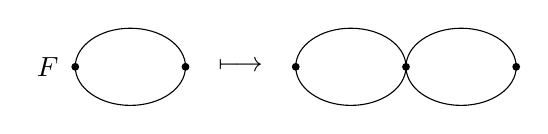
\begin{tikzpicture}[scale=0.7]
          \node at (-6.5, 0) {$F$};
          \draw (-5,0) ellipse (1cm and 0.7cm);
          \node [dot] at (-6,0) {};
          \node [dot] at (-4,0) {};
          \node at (-3, 0) {$\longmapsto$};
          \draw (-1,0) ellipse (1cm and 0.7cm);
          \draw (1,0) ellipse (1cm and 0.7cm);
          \node [dot] at (0,0) {};
          \node [dot] at (-2,0) {};
          \node [dot] at (2,0) {};
        \end{tikzpicture}
      \end{center}
    \item $\{\bot, \top\}$ is initial object in $\mathbf{BiP}$
    \item Dyadic rationals in $[0,1]$ are initial algebra
  \end{itemize}
\end{frame}
\begin{frame}
  \frametitle{Real interval}
  \begin{itemize}
    \item Category of intervals: linearly ordered sets with least and greatest element
    \item Same functor: glue the greatest element of the first copy to the least element of the second copy
    \item $F: [0,1] \mapsto [0,1] \vee [0,1] \cong [0,2]$
      \begin{equation*}
        \begin{tikzcd}[ampersand replacement=\&]
          A \rar \dar \& \left[0,1\right] \dar \\
          A \vee A \rar \& {\left[0,2\right]}
        \end{tikzcd}
      \end{equation*}
      \begin{equation*}
        0.x_1 \dotsm x_n 011111\dotsm = 0.x_1 \dotsm x_n 100000\dotsm
      \end{equation*}
  \end{itemize}
\end{frame}
\end{document}
